%!TEX program=xelatex
%!TEX spellcheck=en_US
\documentclass[final]{report}
% Include all project wide packages here.
%\usepackage{fullpage}
\usepackage[a4paper,margin=4cm,top=2cm,bottom=3cm]{geometry}
\usepackage{polyglossia}
\setmainlanguage{english}
\usepackage{csquotes}
\usepackage{graphicx}
\usepackage{pdfpages}
\usepackage{caption}
\usepackage[list=true]{subcaption}
\usepackage{float}
\usepackage{standalone}
\usepackage{import}
\usepackage{tocloft}
\usepackage{wrapfig}
\usepackage{authblk}
\usepackage{array}
\usepackage{booktabs}
\usepackage[title,titletoc]{appendix}
\usepackage{fontspec}
\usepackage{pgfplots}
\usepackage{tikz}
\usepackage[binary-units=true,parse-numbers=true,table-auto-round=true]{siunitx}
\DeclareSIUnit\flops{FLOPS}
\DeclareSIUnit\iops{IOPS}
\sisetup{detect-weight=true}
\usepackage{units}
\usepackage{amsmath}
\usepackage{mathtools}
\usepackage{unicode-math}
\usepackage{rotating}
\usepackage[compact]{titlesec}
\usepackage{titletoc}
\usepackage{blindtext}
\usepackage{color}
\usepackage{enumitem}
\usepackage{tabularx}
\usepackage{titling}
\usepackage[%
siunitx,
fulldiodes,
europeanvoltages,
europeancurrents,
europeanresistors,
americaninductors,
smartlabels]{circuitikz}

\usetikzlibrary{calc}
\usetikzlibrary{positioning}
\usetikzlibrary{automata}
\usetikzlibrary{arrows.meta}

\tikzstyle{every state}=[fill=tu-cyan,align=center,draw=black,line width=1pt,node distance=3cm,minimum width = 1.8cm]%for FSMs casper
\tikzstyle{every initial by arrow}=[initial text={Reset}]
\newcommand{\setpathasarrows}{\tikzstyle{every path}=[auto,line width=1.5pt,line cap=round,line join=round]}

\pgfplotsset{compat=newest}
\pgfplotsset{plot coordinates/math parser=false}
\usetikzlibrary{plotmarks}
\usepgfplotslibrary{patchplots}
\newlength\figureheight
\newlength\figurewidth

\usepackage[
%backend=bibtex,
backend=biber,
	texencoding=utf8,
bibencoding=utf8,
style=numeric,
citestyle=numeric,
    sortlocale=en_US,
    language=auto,
    backref=true,
    abbreviate=false,
    date=iso8601
]{biblatex}


\usepackage{listings}
\newcommand{\includecode}[4][c]{\lstinputlisting[caption=#2, escapechar=, style=#1,label=#4]{#3}}
\newcommand{\superscript}[1]{\ensuremath{^{\textrm{#1}}}}
\newcommand{\subscript}[1]{\ensuremath{_{\textrm{#1}}}}


\newcommand{\chapternumber}{\thechapter}
\renewcommand{\appendixname}{Appendix}
\renewcommand{\appendixtocname}{Appendices}
\renewcommand{\appendixpagename}{Appendices}


\setlist[enumerate]{labelsep=*, leftmargin=1.5pc}
\setlist[enumerate,1]{label=\arabic*., ref=\arabic*}
\setlist[enumerate,2]{label=\arabic*.,ref=\theenumi.\arabic*}
\setlist[enumerate,3]{label=\arabic*., ref=\theenumii.\arabic*}

\usepackage{xr-hyper}
\usepackage[hidelinks]{hyperref} %<--------ALTIJD ALS LAATSTE
\usepackage[nameinlink,noabbrev,capitalise]{cleveref} %<------- Clever Ref moet na hyperref
\crefname{app}{Appendix}{Appendices}
%\renewcommand{\familydefault}{\sfdefault}


\setmainfont{Myriad Pro}[Ligatures={Common,TeX}]
%\setmathfont{Asana Math}
\setmathfont{Asana-Math.otf}
\setmonofont[Scale=0.9]{Lucida Console}
\newfontfamily\headingfont{Minion Pro}[Ligatures={Common,TeX}]


%Design colors
\definecolor{accent1}{RGB}{0,100,200}
\definecolor{accent2}{RGB}{0,50,100}
\definecolor{tu-cyan}{RGB}{0,166,214}

\newcommand{\hsp}{\hspace{20pt}}
\titleformat{\chapter}[hang]{\Huge\headingfont}{\chapternumber\hsp\textcolor{accent2}{|}\hsp}{0pt}{\Huge\headingfont}

\titleformat{name=\chapter,numberless}[hang]{\Huge\headingfont}{\hsp\textcolor{accent2}{|}\hsp}{0pt}{\Huge\headingfont}

\titleformat{\section}[block]{\LARGE\headingfont}{\arabic{chapter}.\arabic{section}}{0.4em}{}
\titleformat{\subsection}[block]{\Large\headingfont}{\arabic{chapter}.\arabic{section}.\arabic{subsection}}{0.4em}{}
\titleformat{\subsubsection}[block]{\large\headingfont}{\arabic{chapter}.\arabic{section}.\arabic{subsection}.\arabic{subsubsection}}{0.4em}{}
\renewcommand{\arraystretch}{1.25}
\renewcommand{\baselinestretch}{1.25}

\renewcommand\cfttoctitlefont{\headingfont\Huge}
\renewcommand\cftloftitlefont{\headingfont\Huge}
\renewcommand\cftlottitlefont{\headingfont\Huge}
\setcounter{lofdepth}{2}
\setcounter{lotdepth}{2}


\setlength{\parindent}{0pt}
\setlength{\parskip}{0.75em}


%SIuntix settings:
%default: 0V to 10V
%custom: 0 - 10V
\sisetup{range-phrase=--}
\sisetup{range-units=single}
\DeclareSIUnit\years{years}

%For code listings
\definecolor{black}{rgb}{0,0,0}
\definecolor{browntags}{rgb}{0.65,0.1,0.1}
\definecolor{bluestrings}{rgb}{0,0,1}
\definecolor{graycomments}{rgb}{0.4,0.4,0.4}
\definecolor{redkeywords}{rgb}{1,0,0}
\definecolor{bluekeywords}{rgb}{0.13,0.13,0.8}
\definecolor{greencomments}{rgb}{0,0.5,0}
\definecolor{redstrings}{rgb}{0.9,0,0}
\definecolor{purpleidentifiers}{rgb}{0.01,0,0.01}


\lstdefinestyle{csharp}{
language=[Sharp]C,
showspaces=false,
showtabs=false,
breaklines=true,
showstringspaces=false,
breakatwhitespace=true,
escapeinside={(*@}{@*)},
columns=fullflexible,
commentstyle=\color{greencomments},
keywordstyle=\color{bluekeywords}\bfseries,
stringstyle=\color{redstrings},
identifierstyle=\color{purpleidentifiers},
basicstyle=\ttfamily\small}

\lstdefinestyle{c}{
language=C,
showspaces=false,
showtabs=false,
breaklines=true,
showstringspaces=false,
breakatwhitespace=true,
escapeinside={(*@}{@*)},
columns=fullflexible,
commentstyle=\color{greencomments},
keywordstyle=\color{bluekeywords}\bfseries,
stringstyle=\color{redstrings},
identifierstyle=\color{purpleidentifiers},
}

\lstdefinestyle{cpp}{
language=C++,
showspaces=false,
showtabs=false,
breaklines=true,
showstringspaces=false,
breakatwhitespace=true,
escapeinside={(*@}{@*)},
columns=fullflexible,
commentstyle=\color{greencomments},
keywordstyle=\color{bluekeywords}\bfseries,
stringstyle=\color{redstrings},
identifierstyle=\color{purpleidentifiers},
}

\lstdefinestyle{matlab}{
language=Matlab,
showspaces=false,
showtabs=false,
breaklines=true,
showstringspaces=false,
breakatwhitespace=true,
escapeinside={(*@}{@*)},
columns=fullflexible,
commentstyle=\color{greencomments},
keywordstyle=\color{bluekeywords}\bfseries,
stringstyle=\color{redstrings},
identifierstyle=\color{purpleidentifiers}
}

\lstdefinestyle{vhdl}{
language=VHDL,
showspaces=false,
showtabs=false,
breaklines=true,
showstringspaces=false,
breakatwhitespace=true,
escapeinside={(*@}{@*)},
columns=fullflexible,
commentstyle=\color{greencomments},
keywordstyle=\color{bluekeywords}\bfseries,
stringstyle=\color{redstrings},
identifierstyle=\color{purpleidentifiers}
}

\lstdefinestyle{xaml}{
language=XML,
showspaces=false,
showtabs=false,
breaklines=true,
showstringspaces=false,
breakatwhitespace=true,
escapeinside={(*@}{@*)},
columns=fullflexible,
commentstyle=\color{greencomments},
keywordstyle=\color{redkeywords},
stringstyle=\color{bluestrings},
tagstyle=\color{browntags},
morestring=[b]",
  morecomment=[s]{<?}{?>},
  morekeywords={xmlns,version,typex:AsyncRecords,x:Arguments,x:Boolean,x:Byte,x:Char,x:Class,x:ClassAttributes,x:ClassModifier,x:Code,x:ConnectionId,x:Decimal,x:Double,x:FactoryMethod,x:FieldModifier,x:Int16,x:Int32,x:Int64,x:Key,x:Members,x:Name,x:Object,x:Property,x:Shared,x:Single,x:String,x:Subclass,x:SynchronousMode,x:TimeSpan,x:TypeArguments,x:Uid,x:Uri,x:XData,Grid.Column,Grid.ColumnSpan,Click,ClipToBounds,Content,DropDownOpened,FontSize,Foreground,Header,Height,HorizontalAlignment,HorizontalContentAlignment,IsCancel,IsDefault,IsEnabled,IsSelected,Margin,MinHeight,MinWidth,Padding,SnapsToDevicePixels,Target,TextWrapping,Title,VerticalAlignment,VerticalContentAlignment,Width,WindowStartupLocation,Binding,Mode,OneWay,xmlns:x}
}

\lstdefinestyle{python}{
language=Python,
showspaces=false,
showtabs=false,
breaklines=true,
showstringspaces=false,
breakatwhitespace=true,
escapeinside={(*@}{@*)},
columns=fullflexible,
commentstyle=\color{greencomments},
keywordstyle=\color{bluekeywords}\bfseries,
stringstyle=\color{redstrings},
identifierstyle=\color{purpleidentifiers},
}

%defaults
\lstset{
basicstyle=\ttfamily\scriptsize ,
extendedchars=false,
numbers=left,
numberstyle=\ttfamily\tiny,
stepnumber=1,
tabsize=4,
numbersep=5pt
}
\addbibresource{../../.library/bibliography.bib}
\begin{document}
\chapter{Results}
To start off, the same trends were spotted as in Lab 1 and therefore all the benchmarks are run with a local block size of 16x16, or smaller with a smaller problem size.
The global block size will be adjusted to fit the problem size, the standard problem size is 64x64 unless specified otherwise.

Another thing to note, is that the copying of the output data was turned off for the benchmarking.
This greatly improved speed and didn't affect the relative time difference between CUDA and OpenCL.
The CPU performance on the other hand will turn out to be a bit more positive when output generation is turned on, since it does not have to copy the data back from a remote device.
On the other hand, the CPU code runs so slow that its number of simulation steps is 20 times lower than that of CUDA and OpenCL.
The CPU comparison is taken up in the report merely to verify and learn more about its performance, however actually all the running times of the CPU should be multiplied by 20.
It is by no means a close match between the CPU and GPU.

\section{Execution Time for different Enhancements}
\cref{tab:results}, lists the results for the three enhancement stages.
The timing of the CUDA and CPU code is not very reliable.
Basically, the time should be the same for each stage, since the CPU and CUDA code did not receive any edits in between the stages.
During the benchmarking several IO stalls and some other unidentified problems occurred and multiple runs were not able to filter out several runtime spikes.
Therefore, the spikes of both the CPU and CUDA are filtered out by taking the average of the other two correct values.

\begin{table}[H]
	\centering
	\caption{Benchmarking results, total and kernel time for CPU, CUDA and OpenCL}
	\label{tab:results}
	\begin{tabular}{ccccccc}
		\toprule
			\textbf{Stage}		& \textbf{CPU Tot.}	& \textbf{CUDA Tot.}	& \textbf{OpenCL Tot.}	& \textbf{CPU Ker.}	& \textbf{CUDA Ker.}	& \textbf{OpenCL Ker.}\\
		\midrule
			\textit{Stage 1}	& 77.1 (s)			& 56.7 (6.36)			& 18.8 (s) 				& 37.1 (s) 			& 1.92 (6.3)			& 14.5 (s)	\\
			\textit{Stage 2}	& 77.5 (s)			& 6.4 (s) 				& 19.4 (s) 				& 37.4 (s) 			& 6.4 (s) 				& 15.2 (s)	\\
			\textit{Stage 3}	& 54.3 (77.3)		& 6.32 (s) 				& 16.4 (s) 				& 40.3 (37.2) 		& 6.3 (s) 				& 12.5 (s)	\\
		\bottomrule
	\end{tabular}
\end{table}

As mentioned in \cref{sec:iapp-array}, transforming \texttt{iApp} into an array will not contribute to the performance.
Therefore, only the image texture can make a difference in stage 2, this should help speeding up edge conditions for the neighbour computations.
However, the image texture a drop in performance of 0.7 sec (5\% drop).
This is very likely due to the many typecasts that needed to be done, as described in \cref{sec:image-texture}, to make use of this feature in OpenCL.
Hence, one can conclude that both enhancements will not be transferred to Stage 3.

Stage 3 explores the option of merging the neighbour and compute kernel into one.
This allows for more efficient passing of values, and prevent any kernel swapping (intensive operation).
This enhancement proves to be a good choice and a 16\% performance increase is seen.

\begin{figure}[H]
\centering
    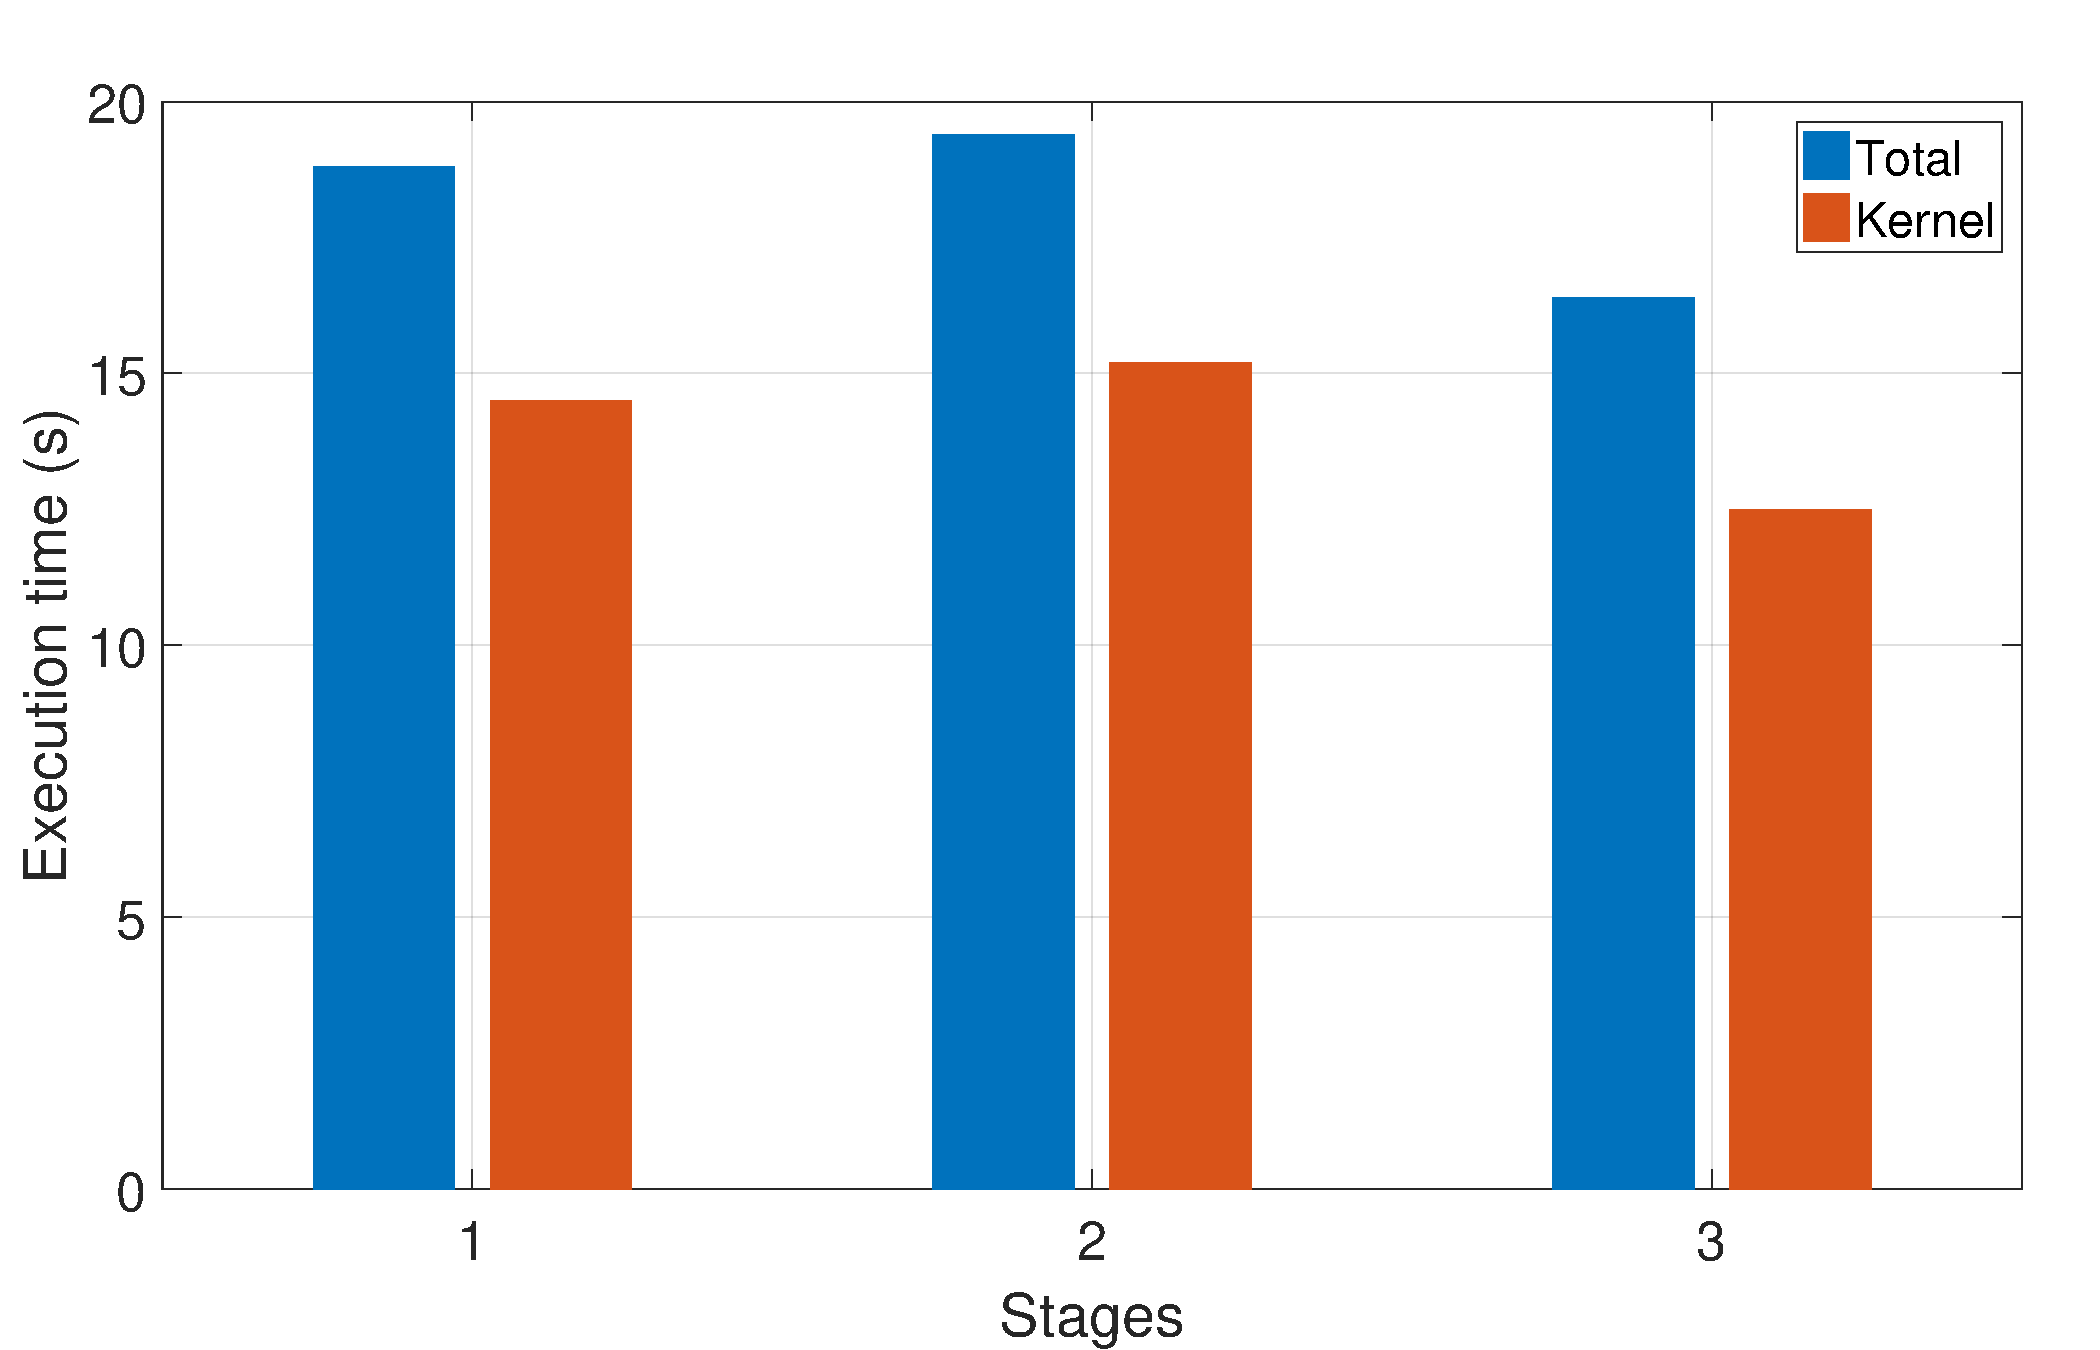
\includegraphics[width=\textwidth]{resources/opencl-per-stage-graph.pdf}
    \caption{The kernel execution time per enhancement stage for OpenCL}
    \label{fig:opencl-per-stage-graph}
\end{figure}

\cref{fig:opencl-per-stage-graph}, shows the execution time of each stage for the total and kernel time.
The total and kernel time always keep the same relative gap to each other.
This indicates that the total time is actually only affected by the kernel time.
This is obvious, since the enhancement stages mainly focused on improving the kernel time and the data needs to be copied to the GPU anyways.


\section{Execution Time for different Problem Sizes}
The section above shows that the maximum speed can be achieved with the Stage 3 enhancements.
To gain some more insight into the performance of the final configuration, the OpenCL code is tested against the CPU and CUDA code for different problem sizes.

\begin{table}[H]
	\centering
	\caption{Benchmarking results, total and kernel time for CPU, CUDA and OpenCL for different problem sizes ranging from 8x8 to 512x512}
	\label{tab:results-problem-size}
	\begin{tabular}{ccccccc}
		\toprule
			\textbf{Size}		& \textbf{CPU Tot.}	& \textbf{CUDA Tot.}	& \textbf{OpenCL Tot.}	& \textbf{CPU Ker.}	& \textbf{CUDA Ker.}	& \textbf{OpenCL Ker.}\\
		\midrule
			8					& 0.84 (s)			& 3.02 (s)				& 14.41 (s)				& 0.62 (s)			& 3.02 (s)				& 10.52 (s) \\
			16					& 3.38 (s)			& 2.93 (s)				& 15.56 (s)				& 2.51 (s)			& 2.93 (s)				& 11.68 (s) \\
			32					& 13.46 (s)			& 3.10 (s)				& 15.57 (s)				& 9.99 (s)			& 3.10 (s)				& 11.69 (s) \\
			64					& 53.81 (s)			& 6.32 (s)				& 16.31 (s)				& 39.94 (s)			& 6.32 (s)				& 12.44 (s) \\
			128					& 220.11 (s)		& 31.03 (s)				& 32.89 (s)				& 164.86 (s)		& 31.02 (s)				& 29.00 (s) \\
		\bottomrule
	\end{tabular}
\end{table}

\cref{tab:results-problem-size}, lists the results for the different problem sizes.
As expected, the execution time of the CPU grows quadratically and after 256x256 the run timed out. 
The performance of the CUDA and OpenCL code is much more interesting.
According to \cref{tab:gpu-specs}, the GPU has 2880 cores.
This means that for a size of roughly 53x53 the kernel execution time should hardly grow, since all computations can be done in parallel below this size.
\cref{fig:exe-time-per-problem-size-graph} and \cref{fig:kernel-time-per-problem-size-graph}, both confirm this, as the execution time starts to grow after a size of 32x32.

\begin{figure}[H]
\centering
    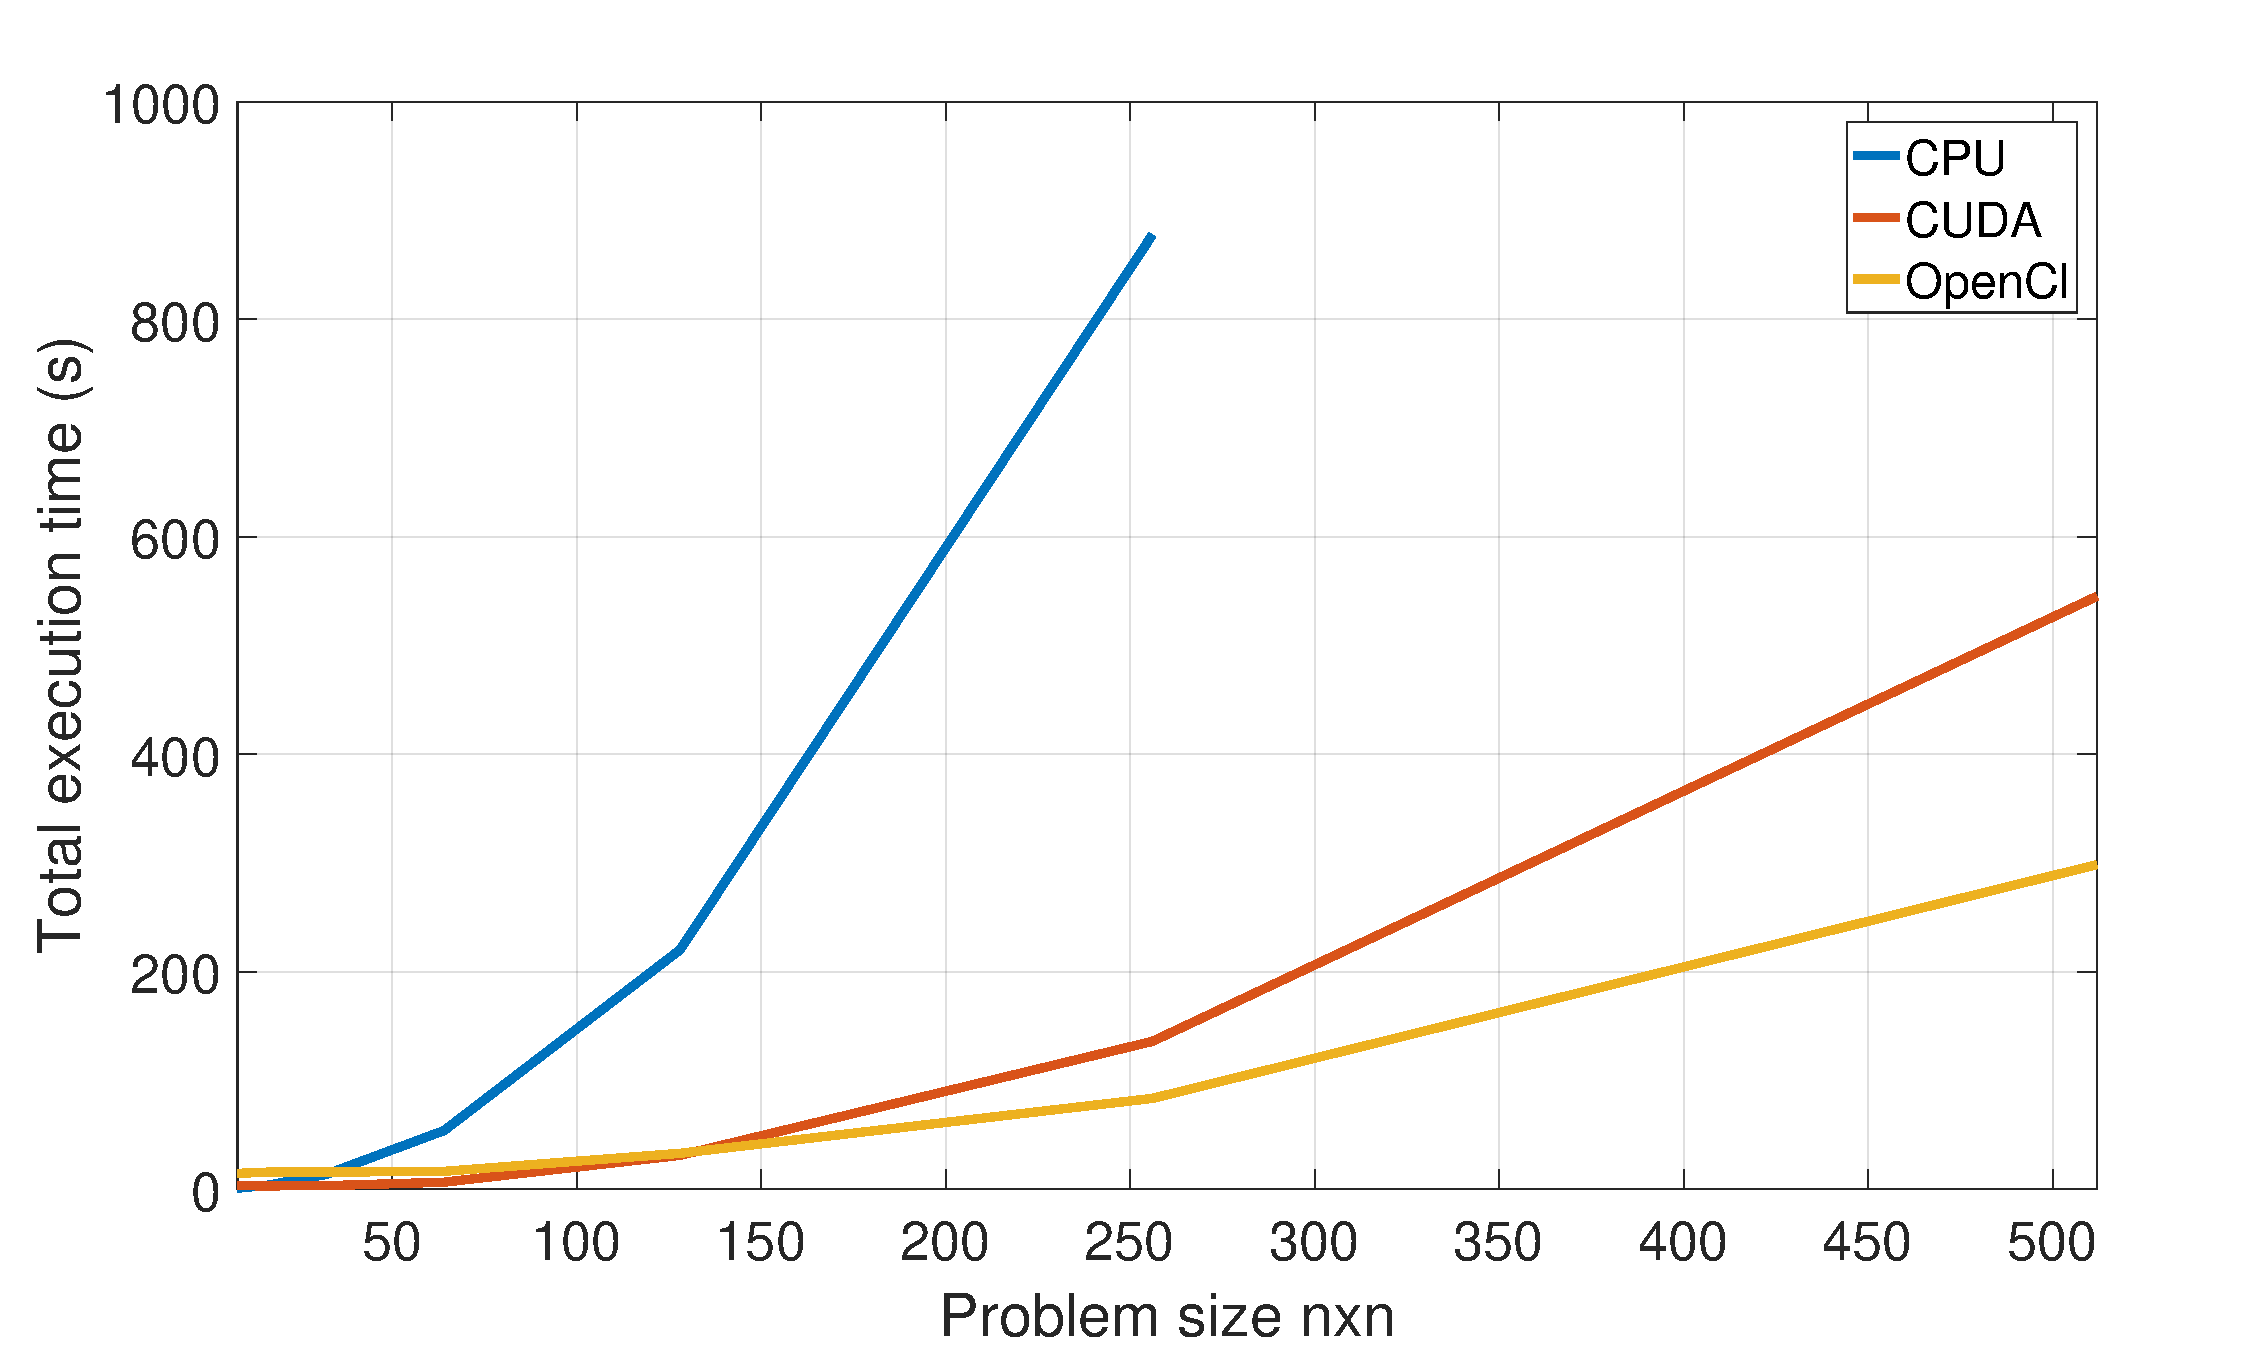
\includegraphics[width=\textwidth]{resources/exe-time-per-problem-size-graph.pdf}
    \caption{The total time for different problem sizes}
    \label{fig:exe-time-per-problem-size-graph}
\end{figure}

\begin{figure}[H]
\centering
    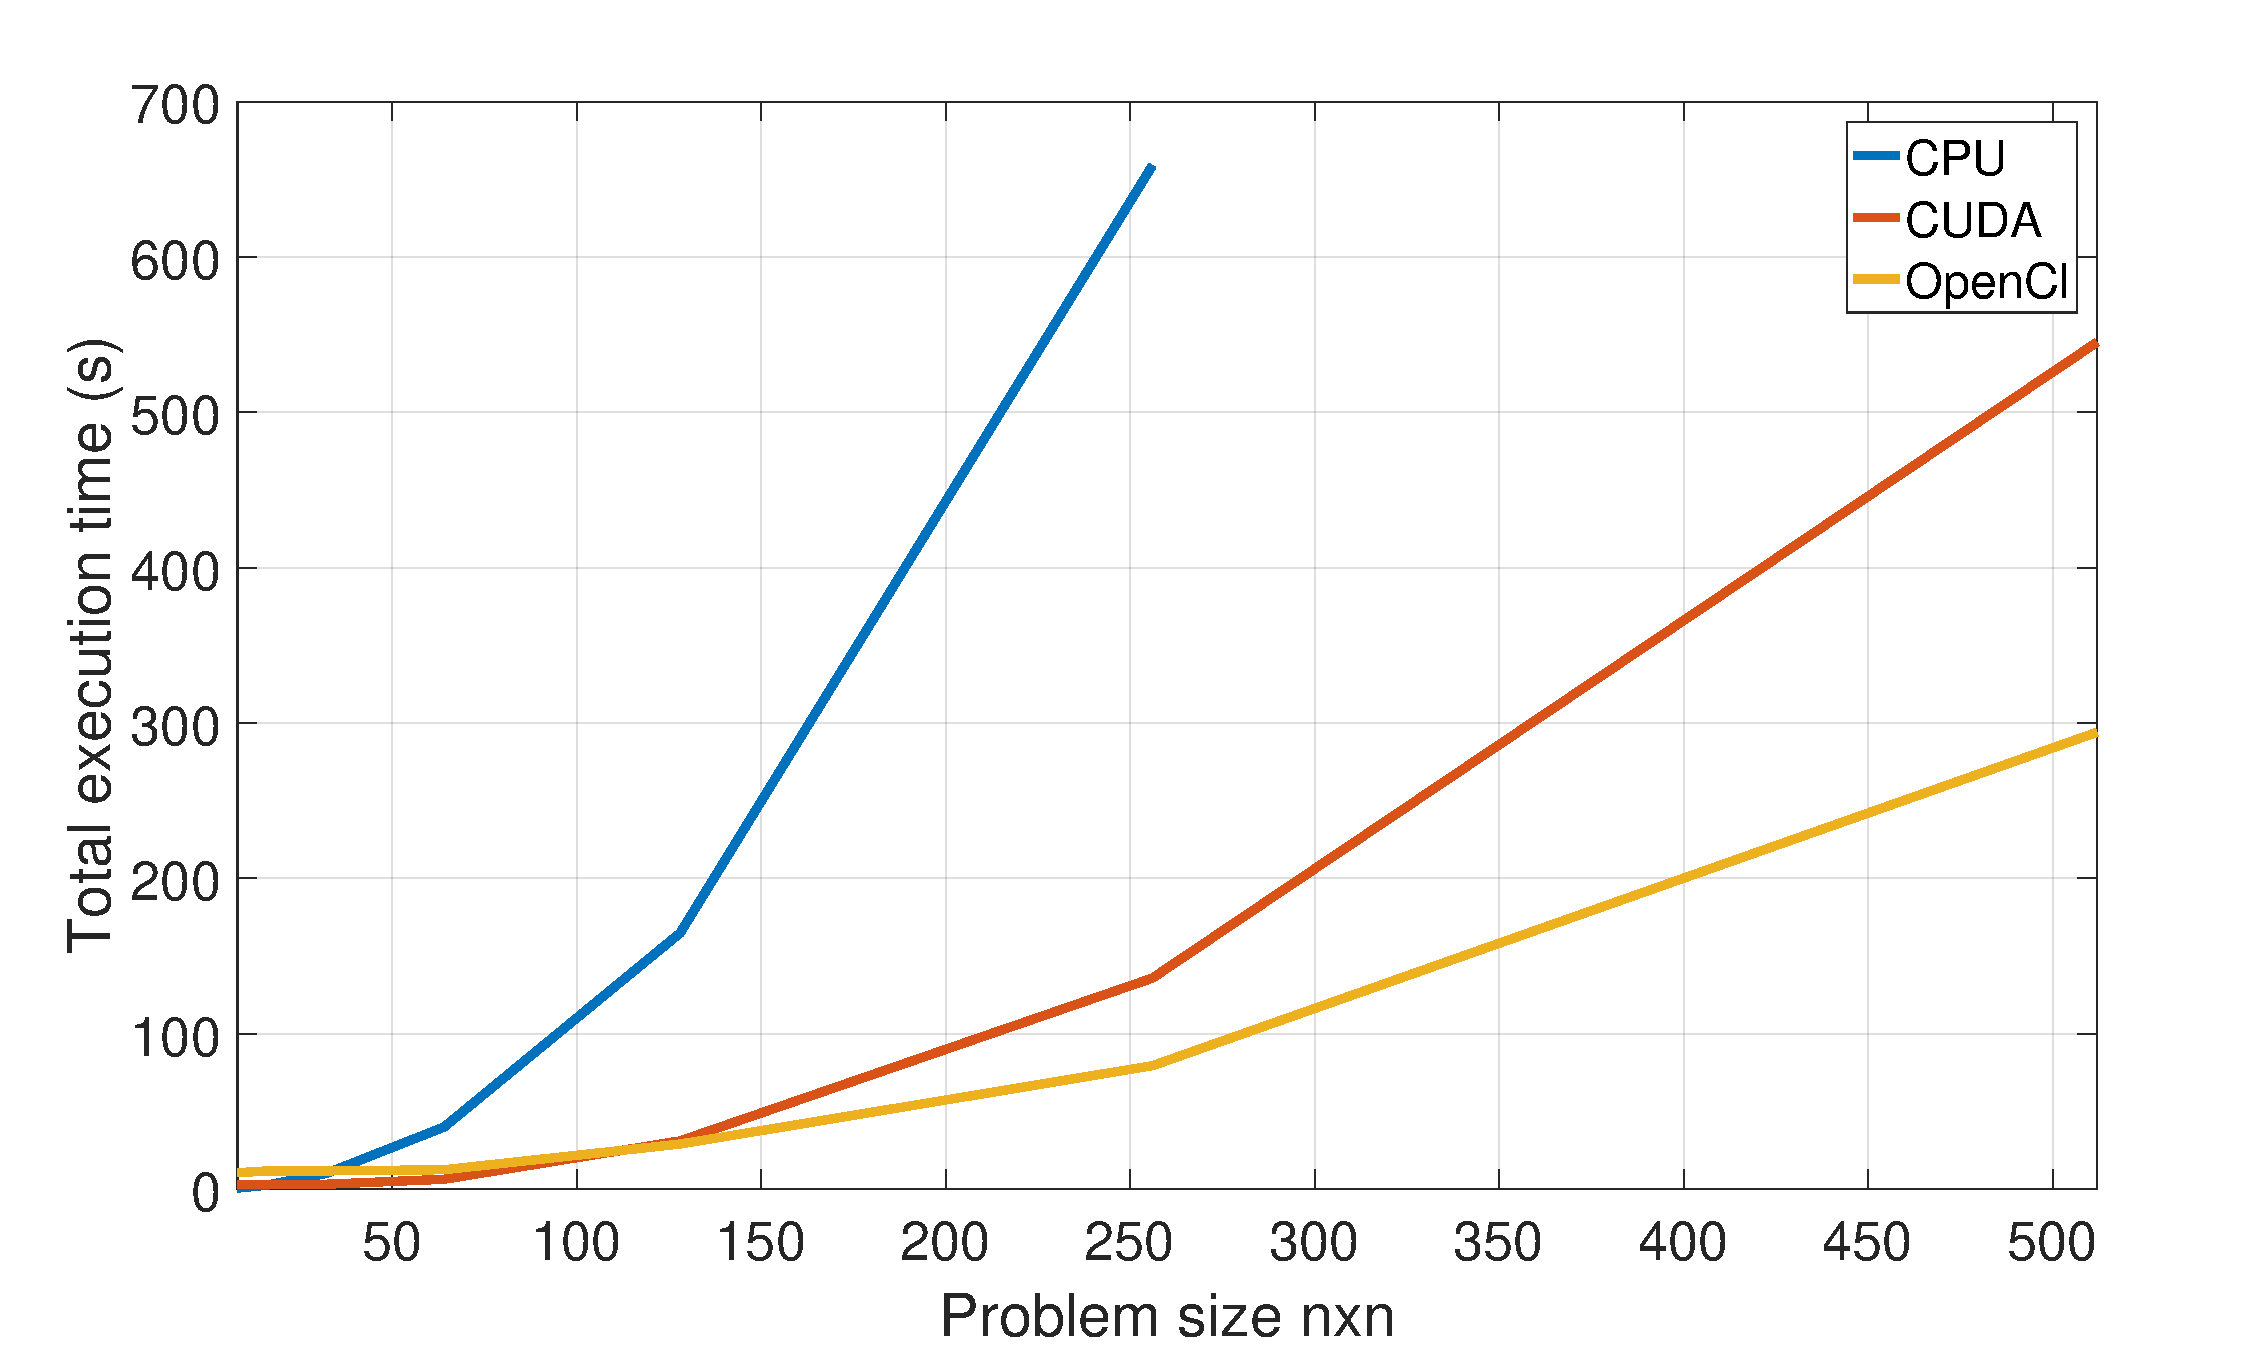
\includegraphics[width=\textwidth]{resources/kernel-time-per-problem-size-graph.pdf}
    \caption{The kernel time for different problem sizes}
    \label{fig:kernel-time-per-problem-size-graph}
\end{figure}

A very interesting investigation is that after a size of 128x128, OpenCL starts to overtake CUDA in terms of performance.
A reason for this could be that the OpenCL kernel is faster for all problem sizes, but that the kernel startup time is hiding this.
For bigger problem size, the kernel startup starts to contribute less to the execution time and the actual performance of the kernel starts to show itself more.
From these results must be concluded that the OpenCL Stage 3 kernel is faster than the CPU and CUDA implementation. 

\end{document}